\begin{sectionblock}{Multiple Textbooks}

  Tagging an open-source textbook with the
  CuratedCourses taxonomy enables the margin to be populated with relevant open
  resources.\vspace{1ex}
  
\vspace{-2ex}\parbox[t][][t]{0.49\textwidth}{\begin{center}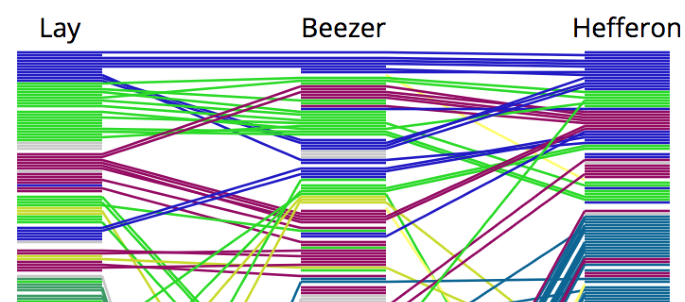
\includegraphics[width=0.45\textwidth,valign=t]{alignment.pdf}\end{center}}\parbox[t][][t]{0.49\textwidth}{\begin{flushleft}And not only can resources be aligned to textbooks, but textbooks can also be aligned with each other.\end{flushleft}\vspace{1ex}\begin{center}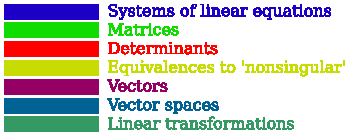
\includegraphics[width=0.49\textwidth]{legend.pdf}\end{center}}


\end{sectionblock}

\vspace{1ex}

\begin{sectionblock}{Workshops and Minicourses}
  As part of the project, the team ran workshops to train
  faculty in the development of and the use of open content, including
  minicourses at the Joint Math Meetings and workshops at participating Universities.


\end{sectionblock}


